% Shared preamble for the English summaries in this repository.
\documentclass[11pt,a4paper]{article}
\usepackage[margin=2.2cm]{geometry}
\usepackage[T1]{fontenc}
\usepackage[utf8]{inputenc}
\usepackage{lmodern}
\usepackage{amsmath,amssymb}
\usepackage{graphicx}
\usepackage{booktabs}
\usepackage{enumitem}
\usepackage[hidelinks]{hyperref}
\setlist{itemsep=2pt,topsep=4pt}
\setlength{\parindent}{0pt}
\setlength{\parskip}{5pt}
\graphicspath{{figures/}}
\newcommand{\summaryheader}[3]{%
  \begin{center}
    {\Large\bfseries #2}\\[3pt]
    {\large #1}\\[3pt]
    {\small Arshia Goshtasbi \textbullet{} MSc Electrical Engineering (Control), Iran University of Science and Technology \textbullet{} #3}
  \end{center}
  \vspace{2pt}\hrule\vspace{8pt}
  \noindent\textit{English summary of my original Persian report, which is kept as a PDF in this folder.}\par}

\begin{document}
\summaryheader{Convex Optimization, Take-home Quiz 4}{Problem Classes: LP, QP, SOCP, SDP}{Spring 1404 (2025)}

\noindent\textit{The code for question 7 is \texttt{Quiz\_Code.m} (YALMIP).}

The quiz asked me to decide whether problems are convex and to rewrite them in a standard form:
\begin{enumerate}
  \item \textbf{Optimality in a QP.} At the optimum $x^\star$ of a convex QP over a feasible set $P$, $-\nabla f(x^\star)$ is a normal to $P$ at $x^\star$: the level set of $f$ just touches the boundary of $P$.
  \item \textbf{Two problems that look hard.} Minimising $\|x\|^2$ outside two discs is not convex, because the feasible set is the complement of a union of discs. Minimising the Gaussian CDF of $c^Tx$ subject to $Ax\le b$, $Hx=g$ is quasi-convex but not convex.
  \item \textbf{A sum of $(|a_i^Tx|-1)^2$.} This objective is not convex. Introducing $p_i=|a_i^Tx|$ and relaxing gives a QP, a QCQP or an SOCP.
  \item \textbf{A piecewise-affine objective.} I split $c^Tx+\max(a_2^Tx+b_2,\ a_3^Tx+b_3)$ into two cases, each an LP.
  \item \textbf{Travel time across two media.} The travel time $T(x)$ from one medium to another (a Snell's-law setting) is convex, which I showed with its second derivative. I extended this to $N$ layers by checking the Hessian.
  \item \textbf{The Bellman equation as an LP.} The value function solves $\min_v \sum_s \mu(s)v(s)$ subject to $v(s)\ge\sum_{s'}P(s'|s,a)[r+\gamma v(s')]$ for all $s,a$.
  \item \textbf{$\min_x \|Ax-b\|_2+\gamma\|x\|_1$ as an SOCP,} with $t\ge\|Ax-b\|_2$ and $-u\le x\le u$. Solved numerically below.
  \item \textbf{$\min\|Ax-b\|_p$.} $p=2$ with complex data becomes a real least-squares problem in $z=[\Re x;\Im x]$. $p=\infty$ and $p=1$ become SOCPs.
  \item \textbf{Bounding a polynomial.} Finding $\inf_t P(t)$ of a polynomial with interval bounds becomes an SDP through a Gram-matrix (sum-of-squares) certificate $P(t)-\gamma=v(t)^TQv(t)$, $Q\succeq 0$.
\end{enumerate}

\section*{Question 7, solved numerically}
\texttt{Quiz\_Code.m} solves question 7 for $A=\begin{bmatrix}1&1\\2&1\\3&2\end{bmatrix}$, $b=(2,3,4)$ and $\gamma=0.5$, then draws the cost contours with the optimum marked.
\IfFileExists{figures/Quiz_Code_1.png}{\begin{center}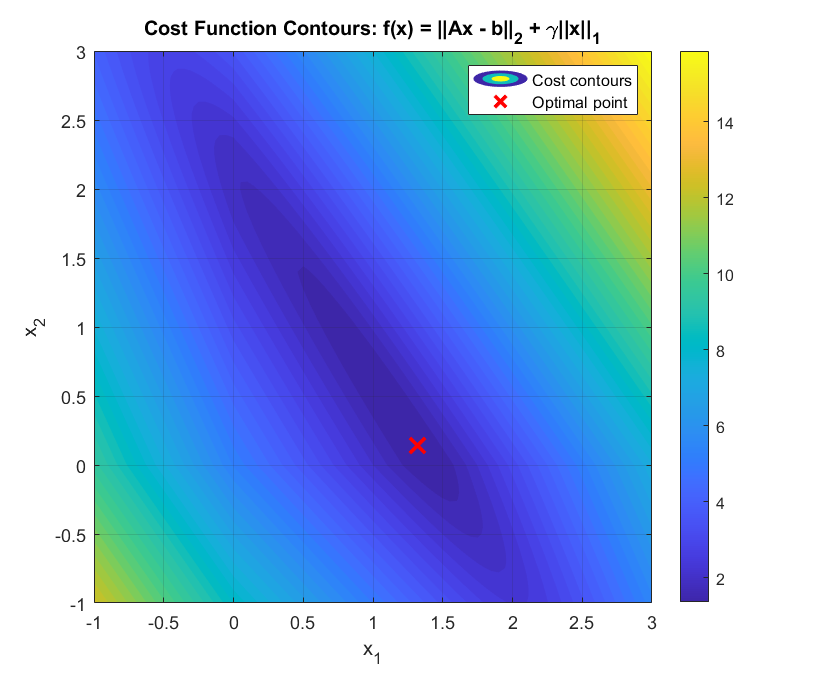
\includegraphics[width=0.6\linewidth]{Quiz_Code_1.png}\end{center}}{}
\end{document}
